\begin{frame}[shrink=10]{\lstinline!rxResponseMaskAnc! - Lato ancora \alert{non} master}
  L'invio delle risposte da parte delle ancore viene regolato dalla maschera \lstinline!rxResponseMaskAnc!.
  Viene mostrato un esempio in cui l'ancora $2$ si comporta da master.
  \begin{columns}
    \begin{column}{0.4\textwidth}
      \begin{center}
        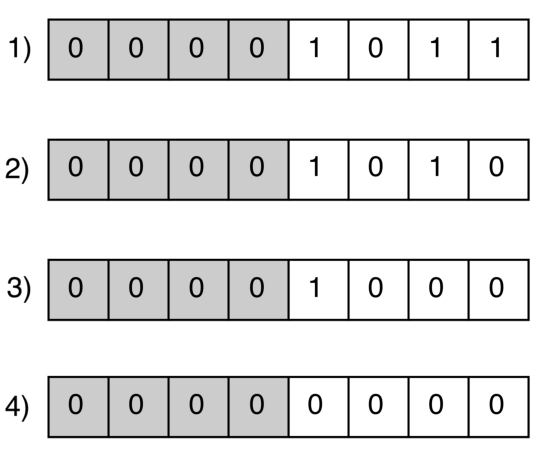
\includegraphics[width=\linewidth]{rxResponseMaskAnc.pdf}
      \end{center}
    \end{column}
    \begin{column}{0.7\textwidth}
      \begin{itemize}
      \item[1)] la maschera viene inizializzata all'arrivo del Poll in tutte le ancore mettendo a $0$ il bit corrispondente alla posizione dell'ancora master
      \item[2)] dopo che l'ancora $0$ ha risposto viene posto a $0$ il bit corrispondente alla posizione dell'ancora 
      \item[3)] dopo che l'ancora $1$ ha risposto viene posto a $0$ il bit corrispondente alla posizione dell'ancora 
      \item[4)] dopo che l'ancora $3$ ha risposto viene posto a $0$ il bit corrispondente alla posizione dell'ancora 
      \end{itemize}
    \end{column}
  \end{columns}
  \begin{exampleblock}{Regola generale}
    E' il turno dell'ancora i-esima di rispondere se il bit in posizione i-esima è il primo diverso da $0$ da destra 
  \end{exampleblock}
\end{frame}

\begin{frame}[shrink = 10]{File instance\_common.c}% - funzioni che gestiscono la maschera \lstinline!rxResponseMaskAnc!}
  \begin{block}{\lstinline!uint8 anch_has_responded()!}
    Restituisce \lstinline!True! se l'istanza ha già risposto altrimenti restituisce \lstinline!False!
  \end{block}
  \begin{block}{\lstinline!uint8 anch_tx_or_wait()!}
    Restituisce \lstinline!True! se l'istanza deve spedire la risposta al tag per poi aggiornare la maschera altrimenti restituisce \lstinline!False!\\
    \textcolor{dgreen}{Attenzione:} l'ancora i-esima deve rispondere se il bit in posizione i-esima della maschera \lstinline!rxResponseMaskAnc! è il primo bit diverso da $0$
    da destra
  \end{block}
  \begin{block}{\lstinline!void handle_rx_mask_on_timout()!}
    Funzione utilizzata per gestire un evento di TimeOut nella procedura di autoranging.\\
    Trova la posizione del primo bit uguale a $1$ nella maschera \lstinline!rxResponseMaskAnc!. La posizione di questo bit corrisponde all'indice dell'ancora che avrebbe
    dovuto inviare la risposta. Successivamente setta il bit a $0$ così da simulare l'avvenuta ricezione del messaggio.
  \end{block}
\end{frame}

\begin{frame}[fragile]{File instance\_common.c}
  \begin{block}{\lstinline!int eval_range(double* range, uint32 tof)!}
    Funzione utilizzata per convertire i tof in distanze espressi in \SI{}{\meter}. Restituisce $0$ se il risultato è negativo o maggiore di \SI{20}{\kilo\meter}, 
    $1$ altrimenti.
  \end{block}
  \begin{block}{\lstinline!void instanceclearcounts()!}
    Viene aggiunta l'inizializzazione di \lstinline!anchRngArray[i]! e \lstinline!tofAnc!
    dove $i$ varia da $0$ a \lstinline!MAX_ANCHOR_LIST_SIZE - 1!
    \begin{lstlisting}
      instance_data[0].anchRngArray[i] = INVALID_TOF;
      instance_data[0].tofAnc = INVALID_TOF;
    \end{lstlisting}
  \end{block}
\end{frame}

\begin{frame}[fragile]{File instance\_common.c}
  \begin{block}{\lstinline!void instanceclearcounts()!}
    Viene inizializzato il numero di volte che il Tag invia la sua posizione al Viewer.
    \begin{lstlisting}
      instance_data[0].tagPositionSentToViewer = 0;
    \end{lstlisting}
    \textcolor{dgreen}{Attenzione:} ogni \lstinline!SEND_ANCHOR_POSITION_EVERY_CYCLES! volte che il tag invia la sua posizione al Viewer tramite seriale viene inviata
    la posizione delle ancore
  \end{block}
  \begin{block}{\lstinline!void instance_set_anch_sleep_delay(int sleepdelay)!}
    Copia in \lstinline!anchSleepTime_ms! il periodo di trasmissione di ogni Poll da parte dell'ancora master
  \end{block}
\end{frame}

\begin{frame}{File instance\_common.c}
  \begin{block}{\lstinline!void enable_tag_polling(instance_data_t *inst)!}
    Inizializza il Tag per la normale procedura di ranging, le istruzioni contenute in questa funzione sono state
    prese dalla parte relativa al Tag del \lstinline!TA_INIT! originale
  \end{block}
\end{frame}

\begin{frame}[fragile]{File instance\_common.c}
  \begin{block}{\lstinline!void instance_backtoanchor(instance_data_t *inst)!}
    Funzione chiamata al termine della procedura di autoranging, oltre a resettare i Timeout
    \begin{lstlisting}
      dwt_setrxtimeout(0);
      dwt_setpreambledetecttimeout(0);
      dwt_setrxaftertxdelay(0);
    \end{lstlisting}
    si occupa di informare l'utente attraverso lo schermo LCD che la procedura di autoranging è terminata
    \begin{lstlisting}
      sprintf((char*)&buff[0], "A:%d AutoRng End", inst->instanceAddress16 & 0x3);
      writetoLCD(16, 1, buff);
    \end{lstlisting}
  \end{block}
\end{frame}

\begin{frame}[fragile]{File instance\_common.c}
  \begin{block}{\lstinline!void eval_means(instance_data_t *inst)!}
    Utilizzata per calcolare le medie dei range accumulati durante la fase di autoranging
    \begin{lstlisting}
      for(i = 0; i < MAX_ANCHOR_LIST_SIZE; i++)
      {
        if(i == (inst->instanceAddress16 & 0x3))
          continue;
        inst->anchRngArray[i] /= inst->anchRngArrayCounter[i];
      }
    \end{lstlisting}
    durante il calcolo della media \alert{non} viene considerato il range di un'ancora con se stessa
  \end{block}
\end{frame}

\begin{frame}[fragile,shrink=30]{File instance\_common.c}
  \begin{block}{\lstinline!void inst_processrxtimeout(instance_data_t *inst)!}
    Gestisce il comportamento dell'ancora master in caso di TimeOut.
    Qualora lo stato precedente fosse \lstinline!TA_TXPOLL_WAIT_SEND! prepara l'ancora all'invio di un nuovo Poll
    \begin{lstlisting}
      inst->instToSleep = TRUE;
      inst->testAppState = TA_TXE_WAIT;
      inst->nextState = TA_TXPOLL_WAIT_SEND;
    \end{lstlisting}
    Qualora lo stato precedente fosse \lstinline!TA_TXFINAL_WAIT_SEND! prepara l'ancora all'invio di un nuovo Poll    
    \begin{lstlisting}
      dwt_forcetrxoff();
      inst->instToSleep = TRUE;
      inst->testAppState = TA_TXE_WAIT;
      inst->nextState = TA_TXPOLL_WAIT_SEND;
    \end{lstlisting}
    Infine gestisce il comportamento dell'ancora \alert{non} master in caso di TimeOut riabilitando immediatamente la ricezione
    \begin{lstlisting}
      inst->testAppState = TA_RXE_WAIT;
      dwt_setrxtimeout(0);
    \end{lstlisting}
  \end{block}
\end{frame}

\begin{frame}[fragile, shirnk=30]{File instance\_common.c}
  \begin{block}{\lstinline!uint8 anc_rx_reenable()!}
    Funzione utilizzata per gestire il comportamento dell'ancora master ad ogni ricezione di un messaggio di risposta.\\
    La maschera \lstinline!mask!
    \begin{lstlisting}
    uint8 mask = (~(0x1 << instance_address)) & 0xF;
    \end{lstlisting}
    viene utilizzata per capire se tutte le ancore hanno risposto ed in quel caso l'istanza si prepara ad inviare il messaggio di Final.\\
    Nel caso in cui solo alcune risposte sono arrivate e \lstinline!instance_data[0].responseTO > 0! viene riconfigurato il TimeOut e riabilitata
    la ricezione 
    \begin{lstlisting}
    dwt_setrxtimeout(fwtoTime_sy * responseTO); 
    dwt_rxenable(DWT_START_RX_IMMEDIATE);
    \end{lstlisting}
  \end{block}
\end{frame}

\begin{frame}{File instance\_common.c}
  \begin{block}{\lstinline!uint8 anc_rx_reenable()!}
    Se, infine, secondo la maschera non tutti hanno risposto ma \lstinline!instance_data[0].responseTO <= 0! viene supposto che l'ultimo messaggio
    arrivato fosse corrotto e viene comunque inviato il Final così da permettere alle ancore che hanno risposto di calcolare il TOF
  \end{block}
  \begin{block}{\lstinline!uint8 anctxorrxreenable(uint16 sourceAddress)!}
    Eliminate le parti realtive alla procedura di autoranging già implementata nel firmware originario della DecaWave
  \end{block}
\end{frame}

\begin{frame}[fragile,shrink=30]{File instance\_common.c}
  \begin{block}{\lstinline!uint8 anc_tx_or_rxreenable_autoranging()!}
    Funzione utilizzata durante la procedura di autoranging dalle ancore non master.
    Qualora tutte le ancore avessero risposto (i.e. \lstinline!instance_data[0].rxResponseMaskAnc == 0!) l'istanza torna nuovamente in ricezione, disabilitando tutti i
    TimeOut, in attesa del messaggio di Final da parte dell'ancora master 
    \begin{lstlisting}
      dwt_setrxtimeout(0);
      dwt_setpreambledetecttimeout(0);
    \end{lstlisting}
    Se, invece è il suo turno di rispondere (i.e. \lstinline!anch_tx_or_wait() == True!) effettua un invio ritardato
    \begin{lstlisting}
      dwt_setdelayedtrxtime(instance_data[0].delayedReplyTime);
      dwt_starttx(DWT_START_TX_DELAYED | DWT_RESPONSE_EXPECTED);
    \end{lstlisting}
    Qualora non fosse ancora il momento di rispondere (i.e. \lstinline!anch_tx_or_wait() == False!) riabilita immediatamente la ricezione
    \begin{lstlisting}
      ancenablerx();
    \end{lstlisting}    
    \textcolor{dgreen}{Attenzione:} dopo aver chiamato \lstinline!anch_tx_or_wait()! la \lstinline!rxResponseMaskAnch! potrebbe essere cambiata ed essere diventata
    nulla, ossia tutti hanno risposto, in tal caso vengono disabilitati i timeout e l'istanza torna nuovamente in ricezione per attendere l'arrivo del messaggio di Final
  \end{block}
\end{frame}

\begin{frame}[fragile]{File instance\_common.c}
  \begin{block}{\lstinline!void handle_error_unknownframe(event_data_t dw_event)!}
    Nel caso in cui il tag sia in modalità \lstinline!TAG_WAIT! gestisce l'arrivo di un messaggio con modalità di indirizzamento
    errata oppure il fatto che \lstinline!rxd->event! sia diverso da \lstinline!DWT_SIG_RX_OKAY! e da \lstinline!DWT_SIG_RX_TIMEOUT!
    La chiamata a questa funzione comporta l'inserimento in coda di un evento di tipo \lstinline!TIMEOUT!)
    \begin{lstlisting}
      dwt_setrxtimeout(0);
      dwt_setpreambledetecttimeout(0);
      ...
      instance_putevent(dw_event, DWT_SIG_RX_TIMEOUT);
    \end{lstlisting}
  \end{block}
\end{frame}

\begin{frame}[fragile,shrink=20]{File instance\_common.c}
  \begin{block}{\lstinline!void ancprepareresponse(uint16 sourceAddress, uint8 srcAddr_index, uint8 fcode_index, uint8 *frame, uint32 uTimeStamp)!}
    E' stata rimossa la parte che gestiva la procedura di autoranging già implementata nel firmware della DecaWave. Vengono inoltre copiate nel messaggio
    di risposta che viene inviato al tag le medie dei range calcolate durante la procedura di autoranging
    \begin{lstlisting}
      for(i = anc_addr + 1, j = 0; i < MAX_ANCHOR_LIST_SIZE; i++, j++)
      {
        uint8 msg_index = AUTORANGING_RANGES + j * sizeof(double);
        memcpy(&(instance_data[0].msg_f.messageData[msg_index]), &instance_data[0].anchRngArray[i], sizeof(double));
      }
    \end{lstlisting}
    \begin{itemize}
    \item[-] l'ancora A$0$ invia i range $r_{0,1}$, $r_{0,2}$ e $r_{0,3}$
    \item[-] l'ancora A$1$ invia i range $r_{1,2}$ e $r_{1,3}$
    \item[-] l'ancora A$2$ invia il range $r_{2,3}$
    \end{itemize}
  \end{block}
\end{frame}

\begin{frame}{File instance\_common.c}
  \begin{block}{\lstinline!void anc_prepare_response_autoranging(uint8 srcAddr_index, uint8 fcode_index, uint8 *frame)!}
    Funzione utilizzata dalle ancore per prerare un messaggio di risposta durante la fase di autoranging.
  \end{block}
\end{frame}

\begin{frame}{File instance\_common.c}
  La funzione \lstinline!void instance_rxcallback(const dwt_callback_data_t *rxd)! ...
\end{frame}

\begin{frame}[fragile]{File instance\_common.c - funzione \lstinline!instance_rxcallback!}
  \begin{block}{fcode \lstinline!RTLS_DEMO_MSG_TAG_POLL!}
    Nel caso in cui un tag sia in modalità \lstinline!TAG_WAIT! inizia la normale procedura di ranging senza aspettare il timeout di $\SI{10}{\second}$
    \begin{lstlisting}
      enable_tag_polling(&instance_data[0]);
      instance_data[0].autoranging_timeout = FALSE;
    \end{lstlisting}
  \end{block}
\end{frame}

\begin{frame}[fragile, shrink=30]{File instance\_common.c - funzione \lstinline!instance_rxcallback!}
  \begin{block}{fcode \lstinline!RTLS_DEMO_MSG_ANCH_POLL!}
    Nel caso in cui un tag sia in modalità \lstinline!TAG_WAIT! sono settati a zero i timeout di ricezione
    \begin{lstlisting}
      dwt_setrxtimeout(0);
      dwt_setpreambledetecttimeout(0);
    \end{lstlisting}
    Nel caso in cui il messaggio sia ricevuto da un'ancora in modalità \lstinline!ANCHOR_RNG! viene settata la maschera
    \lstinline!rxResponseMaskAnc!
    \begin{lstlisting}
      instance_data[0].rxResponseMaskAnc = (~(0x1 << master_anchor)) & 0xF;    
    \end{lstlisting}
    viene preparata la risposta con l'ultimo TOF calcolato
    \begin{lstlisting}
      anc_prepare_response_autoranging(srcAddr_index, fcode_index, &dw_event.msgu.frame[0]);
    \end{lstlisting}
    configurato il timeout 
    \begin{lstlisting}
      dwt_setrxtimeout((uint16)instance_data[0].fwtoTimeAnc_sy);
    \end{lstlisting}
    e gestito l'invio del messaggio
    \begin{lstlisting}
      anc_tx_or_rxreenable_autoranging(instance_data[0].instanceAddress16);
    \end{lstlisting}
  \end{block}
\end{frame}

\begin{frame}[fragile, shrink=50]{File instance\_common.c - funzione \lstinline!instance_rxcallback!}
  \begin{block}{fcode \lstinline!RTLS_DEMO_MSG_ANCH_RESP2!}
    Nel caso in cui un tag sia in modalità \lstinline!TAG_WAIT! sono settati a zero i timeout di ricezione
    \begin{lstlisting}
      dwt_setrxtimeout(0);
      dwt_setpreambledetecttimeout(0);
    \end{lstlisting}
    Nel caso in cui il messaggio sia ricevuto da un'ancora \alert{master} in modalità \lstinline!ANCHOR_RNG! e viene aggiornata la maschera
    e decrementato il contatore
    \begin{lstlisting}
      instance_data[0].responseTO--;
      instance_data[0].rxResponseMaskAnc |= (0x1 << (sourceAddress & 0x3));
    \end{lstlisting}
    Viene inoltre gestito il comportamento dell'ancora \alert{master} (i.e. continua ad aspettare ed invia il messaggio di Final)
    \begin{lstlisting}
      anc_rx_reenable();
    \end{lstlisting}
    Nel caso in cui il messaggio sia ricevuto da un'ancora \alert{non} master in modalità \lstinline!ANCHOR_RNG! la cui maschera sia
    diversa da $0$ (i.e. non sono state ricevute tutte le risposte dalle altre ancore) \lstinline!ANCHOR_RNG! viene aggiornata e l'invio del
    messaggio viene gestito
    \begin{lstlisting}
      instance_data[0].rxResponseMaskAnc &= ~(0x1 << (sourceAddress & 0x3));
      anc_tx_or_rxreenable_autoranging();
    \end{lstlisting}
    Il caso in cui la maschera fosse completamente nulla l'istanza potrebbe non aver ricevuto un messaggio di Poll oppure tutte le risposte sono state già
    ricevute, in questo caso viene resettato il TimeOut e riabilitata immediatamente la ricezione
    \begin{lstlisting}
      dwt_setrxtimeout(0);
      dwt_rxenable(DWT_START_RX_IMMEDIATE);
    \end{lstlisting}
  \end{block}
\end{frame}

\begin{frame}[fragile]{File instance\_common.c - funzione \lstinline!instance_rxcallback!}
  \begin{block}{condizione \lstinline!rxd->event == DWT_SIG_RX_TIMEOUT!}
    Nel caso in cui un'ancora \alert{non} master in modalità \lstinline!ANCHOR_RNG! non abbia ricevuto la risposta attesa e il TimeOut sia scattato viene
    aggiornata la \lstinline!rxResponseMaskAnc! e, nel caso sia arrivato il turno per l'istanza di inviare la risposta, risponde all'ancora master. Così
    da preservare l'interazione tra l'istanza e l'ancora master e calcolare comunque il nuovo TOF
    \begin{lstlisting}
      handle_rx_mask_on_timout();
      anc_tx_or_rxreenable_autoranging();
    \end{lstlisting}
    Viene inoltre generato un evento di tipo \lstinline!DWT_SIG_RX_TIMEOUT!
    \begin{lstlisting}
      instance_putevent(dw_event, DWT_SIG_RX_TIMEOUT);
    \end{lstlisting}
  \end{block}
\end{frame}

\begin{frame}[fragile]{File instance\_common.c}
  \begin{block}{\lstinline!int instance_run()!}
    Nel caso in cui l'uscita della macchina a stati sia \lstinline!INST_DONE_WAIT_FOR_NEXT_EVENT_TO! viene reimpostato il TimeOut per l'invio di un nuovo Poll
    da parte dell'ancora \alert{master}
    \begin{lstlisting}
      nextPeriod = instance_data[0].anchSleepTime_ms;
      instance_data[0].nextSleepPeriod = (uint32) nextPeriod;
    \end{lstlisting}
    Nel caso \lstinline!TAG_WAIT! viene gestito il TimeOut che consente di iniziare la normale procedura di ranging quando
    non viene più rilevata attività di autoranging
    \begin{lstlisting}
      enable_tag_polling(&instance_data[0]);
      instance_data[instance].autoranging_timeout = FALSE;
    \end{lstlisting}
  \end{block}
\end{frame}


    
